% !TEX TS-program = xepythontex



\documentclass[10pt,envcountsect,spanish]{beamer}


\newif\ifnotas
\notasfalse% Para no mostrar los globos
\notastrue % Para  mostrar los globos

\input ../preambulo.tex



%································ TITULO, AUTOR, ETC
\title{Miembros, Sobrecarga y Visibilidad}
\subtitle{Tipos de métodos y variables: Encapsulamiento}


\author[L. Daniel Hernández]{L. Daniel Hernández $<ldaniel@um.es>$}

\institute[ldaniel@um.es]{Dpto. Ingeniería de la Información  y las Comunicaciones\\ Universidad de Murcia \\ \today\newline \hrule}


\date[ldaniel@um.es]{ 
\vskip 1.0cm
%\vskip -1.25cm
%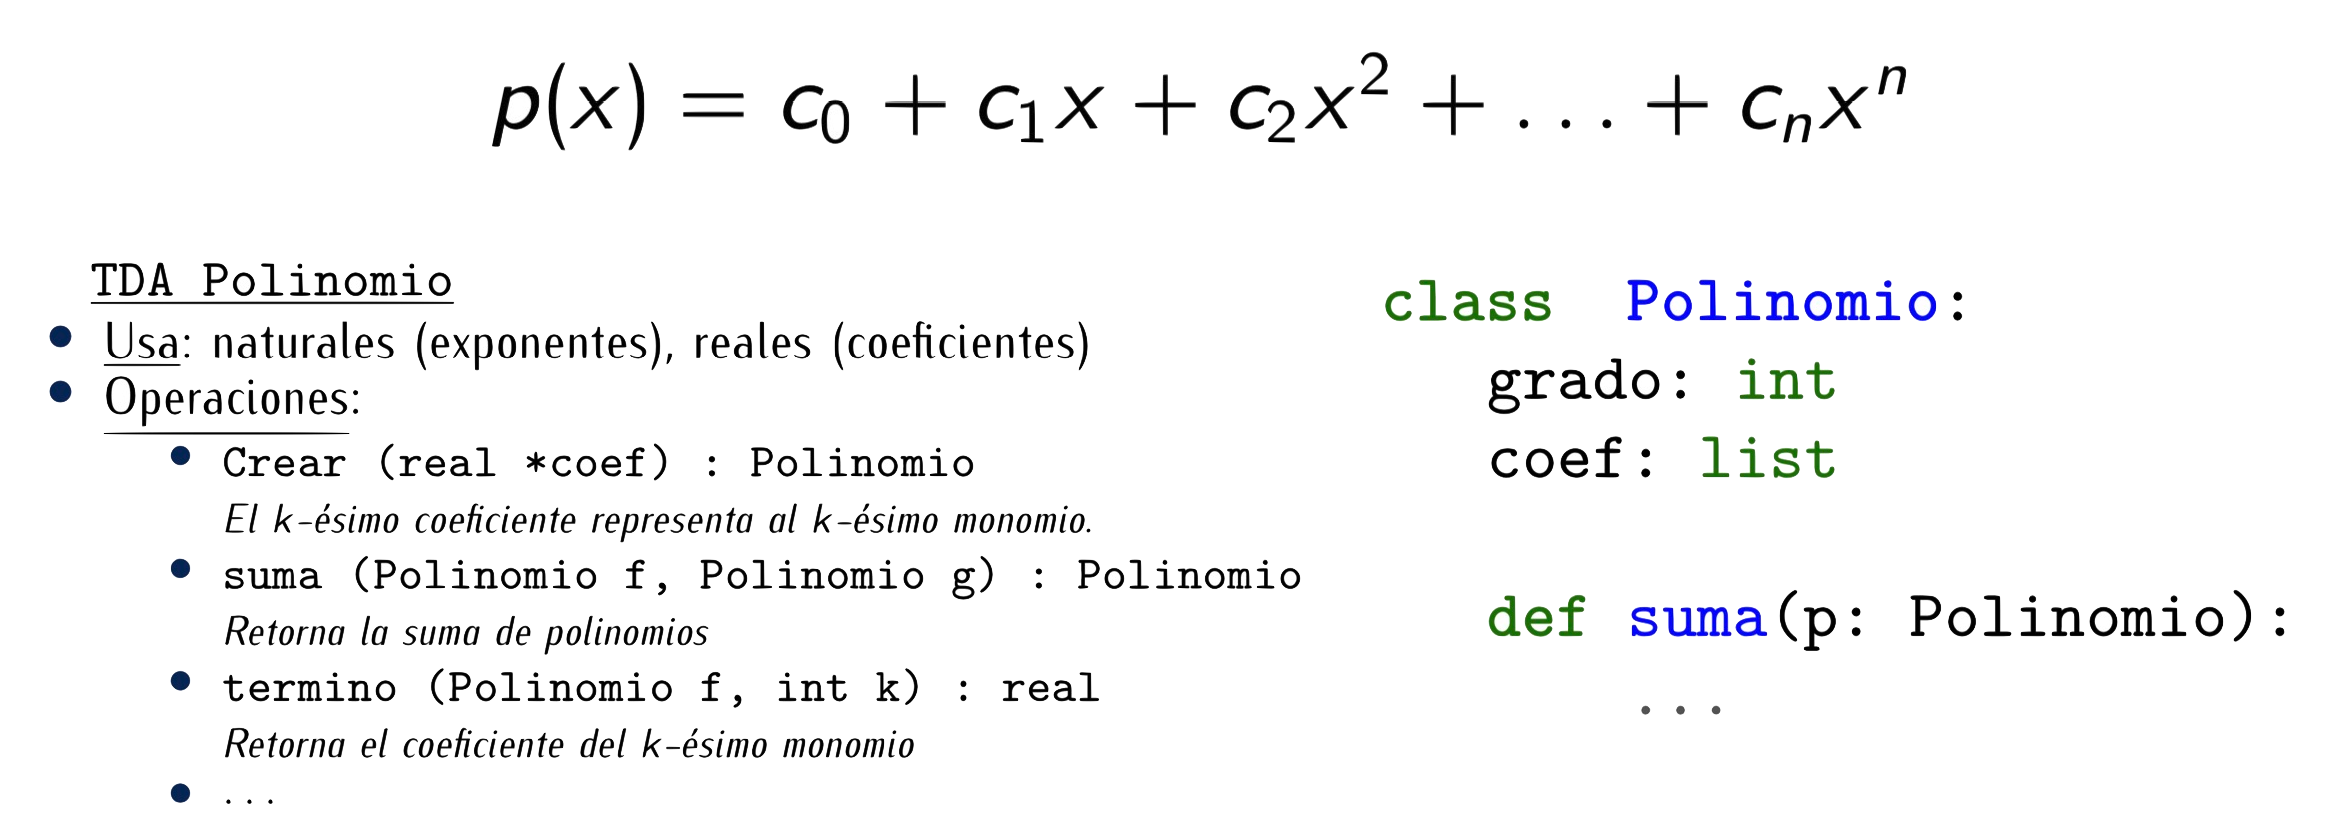
\includegraphics[width=.8\textwidth, height=.18\textheight]{fig/polinomio}
}

\graphicspath{{img/}}



%%%%%%%%%%%%%%%%%%%%%%%%%%%%%%%%%%
%%%%%%%%%%%%%%%%%%%%%%%%%%%%%%%%%%
%%%%%%%%%%%%%%%%%%%%%%%%%%%%%%%%%%
%%%%%%%%%%%%%%%%%%%%%%%%%%%%%%%%%%

%https://es.overleaf.com/learn/how-to/Writing_Markdown_in_LaTeX_Documents
\usepackage[hashEnumerators]{markdown}


%%%%%%%%%%%%%%%%%%%%%%%%%%%%%%%%%%
%%%%%%%%%%%%%%%%%%%%%%%%%%%%%%%%%%
%%%%%%%%%%%%%%%%%%%%%%%%%%%%%%%%%%
%%%%%%%%%%%%%%%%%%%%%%%%%%%%%%%%%%
\begin{document}

%\pgfdeclareimage[height=1cm]{logo}{logo.png}
%\logo{\pgfuseimage{logo}}



%--------------------------------------------------------------------------------
{\usebackgroundtemplate{%
  \includegraphics[width=\paperwidth,height=\paperheight]{../img/fondoUMUCompleto}}
\begin{frame}[b]
	\maketitle

\begin{tikzpicture}[overlay, remember picture]
\node[anchor=south west, %anchor is bottom left corner of the graphic
      xshift=.4\textwidth, %shifting around
      yshift=0.7cm] 
     at (current page.south west) %left bottom corner of the page
     {\includegraphics[width=.4\textwidth, height=.3\textheight]{fig/hombreEscondido}
     \footnote[frame]{\tiny
Imagen: Hombre feliz escondiéndose detrás de la pizarra.
\url{https://www.freepik.es/fotos-premium/hombre-feliz-escondiendose-detras-pizarra_1635302.htm}}}; 
\end{tikzpicture}
	
\end{frame}			% Transparencia: Título
}



%--------------------------------------------------------------------------------
%%%%%%%%%%%%%%%%%%%%%%%%%%%%%%%%%%
%%%%%%%%%%%%%%%%%%%%%%%%%%%%%%%%%%
\begin{frame}{Índice de Contenidos}\tableofcontents \end{frame}


%%%%%%%%%%%%%%%%%%%%%%%%%%%%%%%%%%%%%
%%%%%%%%%%%%%%%  SECTION   %%%%%%%%%%%%%%%
%%%%%%%%%%%%%%%%%%%%%%%%%%%%%%%%%%%%%
\section{Introducción}



%%%%%%%%%%%%%%%%%%%%%%%%%%%%%%%%%%%%%
%%%%%%%%%%%%%%%%%%%%%%%%%%%%%%%%%%%%%
\begin{frame}[fragile]{Introducción} 

\begin{itemize}
\item Una clase representa a un conjunto de objetos, todos ellos con la misma estructura.
\item Una clase consta de una serie de elementos, llamados \key{miembros}.

\begin{code}
class UnaClase {
   miembros
}
\end{code}

\item Los \key{miembros de una clase} son los elementos de una estructura que la caracterizan y, por ende, permite definir a sus objetos.


\item Ya conocemos algunos de sus miembros:
	\begin{itemize}
	\item Las \key{variables}, que definirán el estado de cada objeto.
	\item Los \key{métodos}, que establecen el comportamiento (o funcionalidad) de todos los objetos.
	\end{itemize}

\item Pueden \key{existir otros}: constantes, propiedades, eventos, clases internas, etc.

\item En cada lenguaje de programación los miembros pueden variar.

\item Formalmente, los \key{constructores}, que indican cómo debe establecer el estado inicial de un objeto recién creado, no se consideran miembros de una clase 
	{\small (Realmente hay discusión sobre el tema, que si debe heredarse, que si debe ser estático, ...)}

\item Para todos ellos no se puede permitir que cualquier pueda acceder a cualquier miembro de una clase. 
Hay que imponer restricciones de \key{visibilidad}.
\end{itemize}

\end{frame}
% . . . . . . . . . . . . . . . . . . . . . . . . . . . . . . . . . . . . . . . . . . . . . . . . . . . . . . 
% . . . . . . . . . . . . . . . . . . . . . . . . . . . . . . . . . . . . . . . . . . . . . . . . . . . . . . 

%%%%%%%%%%%%%%%%%%%%%%%%%%%%%%%%%%%%%
%%%%%%%%%%%%%%%  SECTION   %%%%%%%%%%%%%%%
%%%%%%%%%%%%%%%%%%%%%%%%%%%%%%%%%%%%%
\section{Métodos y Variables}


%%%%%%%%%%%%%%%%%%%%%%%%%%%%%%%%%%%%%
%%%%%%%%%%%%%%%  SECTION   %%%%%%%%%%%%%%%
%%%%%%%%%%%%%%%%%%%%%%%%%%%%%%%%%%%%%
\subsection{Métodos}

%%%%%%%%%%%%%%%%%%%%%%%%%%%%%%%%%%%%%
%%%%%%%%%%%%%%%%%%%%%%%%%%%%%%%%%%%%%
\begin{frame}[fragile]{Métodos Miembros} 

\begin{itemize}
\item Hemos indicado que los \key[red]{métodos} representan el \key{comportamiento} de los objetos.
\item Un método está \key{asociado con una acción} que puede realizar un objeto.

\item Siempre se coloca en ``el interior'' de la definición de una clase.

\item[]

\item[] \unEjemplo Pseudocódigo 
\begin{code}[basicstyle=\ttfamily\scriptsize]
class Coche {
   ...
   None recarga (int n) {
      self.gas = n;   // Estable los litros de gas
   } 
   ...
}
\end{code}

	
\item Existen tres tipos de métodos: 
\begin{itemize}
\item \key{de instancia}: uno para todos los objetos.
\item \key{de clase}: uno para toda la clase y común a todos los objetos.
\item \key{estáticos}: es independiente de clases y objetos.
\end{itemize}
\end{itemize}

\end{frame}
% . . . . . . . . . . . . . . . . . . . . . . . . . . . . . . . . . . . . . . . . . . . . . . . . . . . . . . 
% . . . . . . . . . . . . . . . . . . . . . . . . . . . . . . . . . . . . . . . . . . . . . . . . . . . . . . 

%\end{document}



%%%%%%%%%%%%%%%%%%%%%%%%%%%%%%%%%%%%%
%%%%%%%%%%%%%%%%%%%%%%%%%%%%%%%%%%%%%
\begin{frame}[fragile, label={metodoInstancia}]{Métodos de Instancia} 

\begin{itemize}
\item Los \key{métodos de instancia} son los que están asociados a un objeto.
\item Se tiene que invocar \key{a través de un objeto} (existente) de la clase.
\item Se llaman con esta notación punto: \cm{objeto}\cm[blue]{.mombreMétodoInstancia()}
\item \key{Accede a las variables de instancia} (ver pág. \ref{tiposVariables}).
\item En \cm[red]{Python} se reconocen porque tiene como primer parámetro \cm{self} que apunta al objeto que invoca al método.

\centerline{\bf No se recomienda este uso generalizado}

\item[] \unEjemplo  

Los métodos mágicos \pyv{__init__(self, parámetros)} o \pyv{__str__(self)} son ejemplos de métodos de instancia.

\begin{pyverbatim}[][frame=single]
class Rueda:
    def __init__(self, radio):
        self.radio = radio
\end{pyverbatim}
\end{itemize}
\end{frame}
% . . . . . . . . . . . . . . . . . . . . . . . . . . . . . . . . . . . . . . . . . . . . . . . . . . . . . . 
% . . . . . . . . . . . . . . . . . . . . . . . . . . . . . . . . . . . . . . . . . . . . . . . . . . . . . . 


%\end{document}

%%%%%%%%%%%%%%%%%%%%%%%%%%%%%%%%%%%%%
%%%%%%%%%%%%%%%%%%%%%%%%%%%%%%%%%%%%%
\begin{frame}[fragile, label={metodoClase}]{Métodos de Clase} 

\begin{itemize}
\item Los \key{métodos de clase} son los que están asociados a una clase.
\item Se pueden invocar sin existir ningún objeto de la clase.
\item Se usa notación punto: \cm{NombreDeLaClase}\cm[blue]{.nombreMétodoClase()}
\item \textbf{No pueden acceder} a las variables de instancia (ver pág. \ref{tiposVariables}).
\item \key{Operan solo sobre variables de la clase} (afectará a todas las instancias de los objetos), por lo que también se puede usar \cm{objeto}\cm[blue]{.nombreMétodoClase()}
\item En \cm[red]{Python} se reconocen porque tienen el decorador \cm[violet]{\textbf{@classmethod}} y tiene como primer parámetro \cm{cls} que apunta a la clase cuando el método es invocado.


\begin{itemize}
\item Un claro uso de los métodos de clase es usarlos como \key{Funciones Factoría}, que son las que permiten obtener instancias de la clase.
\end{itemize}

\end{itemize}

\unEjemplo 

\footnotesize
\begin{minipage}{.48\textwidth}
\begin{pyconsole}[][frame=single]
class Rueda:
    def __init__(self, radio):
        self.radio = radio
    @classmethod 
    def grande(cls): 
        return cls(500)

\end{pyconsole}
\end{minipage}
\begin{minipage}{.46\textwidth}
\begin{pyconsole}[][frame=single]
# Fabrica una rueda
mi_rueda = Rueda.grande()
# Muestra el radio
print(mi_rueda.radio)
\end{pyconsole}
\end{minipage}
\end{frame}
% . . . . . . . . . . . . . . . . . . . . . . . . . . . . . . . . . . . . . . . . . . . . . . . . . . . . . . 
% . . . . . . . . . . . . . . . . . . . . . . . . . . . . . . . . . . . . . . . . . . . . . . . . . . . . . . 



%%%%%%%%%%%%%%%%%%%%%%%%%%%%%%%%%%%%%
%%%%%%%%%%%%%%%%%%%%%%%%%%%%%%%%%%%%%
\begin{frame}[fragile, label={metodoEstatico}]{Métodos Estáticos} 

\begin{itemize}
\item Los \key{métodos estáticos} son los que no están asociados ni a una clase ni a un objeto.
\item Se pueden invocar sin existir ningún objeto de la clase.
\item Se usa notación punto: \cm{NombreDeLaClase}\cm[blue]{.nombreMétodoEstático()}
\item \key{No pueden acceder ni a las variables de clase ni a las de instancia} (ver pág. \ref{tiposVariables}).
\item Por tanto son métodos independientes de las clases/objetos y útiles para crear métodos ``de utilidad'' (funciones útiles para usar en cualquier momento).
\item En \cm[red]{Python} se reconocen porque tienen el decorador \cm[violet]{@staticmethod}.

\item[]
\unEjemplo Imagina que tienes la clase \cm{Util} que contiene funciones de conversión de medidas. Son útiles porque se podrían usar en cualquier momento (sin depender de un objeto o clase en particular). Serían adecuadas definirlas como métodos estáticos \cm{Util.celsius\_a\_fahrenheit()}, ...
\end{itemize}

\footnotesize
\begin{pyconsole}[][frame=single]
class Rueda:
    @staticmethod
    def superficieAproximada(radio):
        return 3.14*radio**2

Rueda.superficieAproximada(8) # Me valdría para cualquier círculo
\end{pyconsole}
\end{frame}
% . . . . . . . . . . . . . . . . . . . . . . . . . . . . . . . . . . . . . . . . . . . . . . . . . . . . . . 
% . . . . . . . . . . . . . . . . . . . . . . . . . . . . . . . . . . . . . . . . . . . . . . . . . . . . . . 

%\end{document}



%%%%%%%%%%%%%%%%%%%%%%%%%%%%%%%%%%%%%
%%%%%%%%%%%%%%%%%%%%%%%%%%%%%%%%%%%%%
\begin{frame}[fragile]{Algunas aclaraciones} 

\begin{itemize}
\item Hemos distinguido 3 tipos de métodos:
\begin{itemize}
\item Los \key{métodos de instancias} son los que están asociados a un objeto.
\item Los \key{métodos de clase} son los que están asociados a una clase.
\item Los \key{métodos estáticos} son los que \textbf{no} están asociados ni a instancia ni a clases
\end{itemize}

\item Hay lenguajes que distinguen los 3 tipos de métodos. Como en \key[red]{Python}.
\begin{itemize}
\item Los \key{métodos de instancias} tienen como primer parámetro \cm{self}.
\item Los \key{métodos de clase} usa \cm[violet]{@classmethod} y el primer parámetro es  \cm{cls}. 
\item Los \key{métodos estáticos} usa  \cm[violet]{@staticmethod}.
\end{itemize}

\item Hay lenguajes que distinguen solo 2 grupos de métodos. Como en \key[red]{Java}.
\begin{itemize}
\item Los \key{métodos de instancias} son los que \textbf{no tienen} el modificador \cm{static}.
\item Los métodos que sí tienen el modificar static y se pueden interpretar como \key{métodos de clase} o \key{métodos estáticos}. De hecho son términos sinónimos en este lenguaje.
\end{itemize}

\footnotesize
\begin{code}
public class Car {
  public double consumo(double metros) { }  // De instancia
  public static void main(String[] args) { }// Estático. De Clase
}
\end{code}

\end{itemize}

\end{frame}
% . . . . . . . . . . . . . . . . . . . . . . . . . . . . . . . . . . . . . . . . . . . . . . . . . . . . . . 
% . . . . . . . . . . . . . . . . . . . . . . . . . . . . . . . . . . . . . . . . . . . . . . . . . . . . . . 













%%%%%%%%%%%%%%%%%%%%%%%%%%%%%%%%%%%%%
%%%%%%%%%%%%%%%%%%%%%%%%%%%%%%%%%%%%%
\begin{frame}{Ejercicio}


\begin{ejercicio}{}
Indica cómo deberían ser los siguientes métodos (si estáticos, de clase o de instancia)
\begin{itemize}[leftmargin=\dimexpr 1cm]
\item Aplicar una función matemática sobre un número. P.e. \cm{abs()}, \cm{log()}, \cm{sqrt()}, ... % Estático
\item Retornar el número de objetos que se han construido de una clase. % De clase
\item Calcular la suma de dos complejos. % Estático o de instancia.
\end{itemize}
\end{ejercicio}
\end{frame}



%%%%%%%%%%%%%%%%%%%%%%%%%%%%%%%%%%%%%
%%%%%%%%%%%%%%%  SECTION   %%%%%%%%%%%%%%%
%%%%%%%%%%%%%%%%%%%%%%%%%%%%%%%%%%%%%
\subsection{Variables}



%%%%%%%%%%%%%%%%%%%%%%%%%%%%%%%%%%%%%
%%%%%%%%%%%%%%%%%%%%%%%%%%%%%%%%%%%%%
\begin{frame}[fragile, label={fr:objetosMiembros}]{Variables Miembros} 

\begin{itemize}
\item Son \key[red]{variables miembros} las que definen el estado de la \textbf{clases} o sus \textbf{objetos}.
\item También se llaman \key{atributos} o \key{campos}.
\item Pueden ser \key{simples} o \key{compuestas} (p.e. arrays u otros objetos)

\unEjemplo \key[red]{Pseudocódigo}\vskip-0.05cm
%\hskip-0.5cm
\begin{pyverbatim}[][frame=single, fontsize=\scriptsize]
class Persona{
   final String nombrePadre # Estructurado y No cambia (final, constante)
   int edad       # Tipo de Dato simple
   ...
}
class Primitiva {
   int[] numeros  # Estructurado: Array de enteros (TD simple)
   ...
}
class Persona {
   Persona pareja # Estructurado: Objeto (En POO es lo usual)
   ...
}
class Biblioteca {
   Libro[] libros # Estructurado: Array de objetos  (Normal en POO)
   ...
}
\end{pyverbatim}

\item \textbf{No hay que confundir} las \key{variables miembros} con \textbf{otras variables}.
\end{itemize}

\end{frame}
% . . . . . . . . . . . . . . . . . . . . . . . . . . . . . . . . . . . . . . . . . . . . . . . . . . . . . . 
% . . . . . . . . . . . . . . . . . . . . . . . . . . . . . . . . . . . . . . . . . . . . . . . . . . . . . . 












%%%%%%%%%%%%%%%%%%%%%%%%%%%%%%%%%%%%%
%%%%%%%%%%%%%%%%%%%%%%%%%%%%%%%%%%%%%
\begin{frame}[label={tiposVariables}]{Tipos de Variables}

\begin{itemize}
\item Existen 4 tipos de variables: de clase, de instancia, locales y globales
\end{itemize}

\unEjemplo Sobre la clase \key{Estudiante} se pueden definir estas variables:

\begin{itemize}
\item \key{Variables de clase}. Evalúan atributos de toda la clase.
	\begin{itemize}
	\item Número de estudiantes total (varía con el tiempo)
	\item Sistema de calificaciones (constante en el tiempo)
	\item ...	
	\end{itemize}
	
\item \key{Variables de instancia} (u objeto).  Definene el estado para un estudiante:
	\begin{itemize}
	\item Color de los ojos
	\item Referencia al centro en el que estudia
	\item ...
	\end{itemize}
	
\item \key{Variables locales}. Las auxiliares propias de un método, algoritmo, ...
	\begin{itemize}
	\item Las auxiliares para calcular la nota media de un estudiante
	\item Las usadas para ordenar los estudiantes por altura
	\item ...
	\end{itemize}
	
\item \key{Variables globales}. Las que son accesibles por cualquier clase o función.
	\begin{itemize}
	\item El planeta donde viven los estudiantes.
	\item El aire que respiran los estudiantes
	\item ...
	\end{itemize}
\end{itemize}


\end{frame}
% . . . . . . . . . . . . . . . . . . . . . . . . . . . . . . . . . . . . . . . . . . . . . . . . . . . . . . 
% . . . . . . . . . . . . . . . . . . . . . . . . . . . . . . . . . . . . . . . . . . . . . . . . . . . . . . 




%%%%%%%%%%%%%%%%%%%%%%%%%%%%%%%%%%%%%
%%%%%%%%%%%%%%%%%%%%%%%%%%%%%%%%%%%%%
\begin{frame}[fragile,label={varLocalGlobal}]{Varibles Locales y Globales}
\begin{itemize} \setlength\itemsep{0em}
\item El \key{ámbito de una variable} hace referencia a las partes del programa en el que una variable es reconocida.
\item Una variable es \key{local} respecto de un bloque de código si solo es reconocida en ese bloque. Fuera de él, la variables no es reconocida. 

\item Una variable es \key{global} respecto de un bloque de código si se reconoce tanto dentro de dicho bloque como fuera de él.


\item En \cm[red]{Python} se tienen las siguientes situaciones:

\begin{itemize}
\item Variables declaradas ``fuera'' de una función son \key{variables globales} para esa función.

\item Los parámetros de una función/método son variable locales a la función/método

\item Las variables declaradas en el bloque de una función son variables locales a la función.

\item \key{En un bloque todas las variables son locales salvo que se diga lo contrario}
\end{itemize}
\end{itemize}

\footnotesize
\begin{pyconsole}[][frame=single]
s = "global"          # Variable global (está fuera de cualquier función)
def f(param):         # Un parámetro es una variable local
    #global s         # Descomenta !!
    s = "local"       # NO ES REASIGNACIÓN!! - Nueva variable !
    print(s, id(s))
    
f(2)                  # En la invocación s será "local"
print(s, id(s))       # s vale "global"
\end{pyconsole}


\end{frame}

%\end{document}


%%%%%%%%%%%%%%%%%%%%%%%%%%%%%%%%%%%%%
%%%%%%%%%%%%%%%%%%%%%%%%%%%%%%%%%%%%%
\begin{frame}[fragile,label={variablesInstancia}]{Variables de Instancia u Objeto}
\begin{itemize}
\item \key[magenta]{Son variables miembro}
\item Definen el \key{estado} de un objeto.
\item Hay, al menos, tantas como objetos o instancias se hayan creado.
\item Se destruyen cuando se destruye el objeto.
\item Se usa la notación punto: \cm{nombreObjeto}\cm[blue]{.nombreVariable}

\centerline{\textbf{Solo son accesibles a través de un \key[red]{método del} objeto}}

\item Se usan en métodos de instancia (pág \ref{metodoInstancia}).
\item No se pueden usar ni en métodos estáticos ni en métodos de clase (págs \ref{metodoClase}, \ref{metodoEstatico}) Recíprocamente, estos métodos  no te dejará trabajar con este tipo de variables.

\item En \cm[red]{Python} se crea una cada vez que se  realiza una asignación

\begin{pyverbatim}[][frame=single]
self.valor = valor  # P.e. en el método __init__()
objeto.valor = valor # En cualquier lugar
\end{pyverbatim}
Ya que \cm{objeto}\cm[blue]{.valor} se puede realizar en cualquier lugar, \key[red]{se debe usar} \pyv{__slots__ =[variables]} en la definición de la clase para indicar los identificadores permitidos para las variables de instancia.
\end{itemize}
\end{frame}
% . . . . . . . . . . . . . . . . . . . . . . . . . . . . . . . . . . . . . . . . . . . . . . . . . . . . . . 
% . . . . . . . . . . . . . . . . . . . . . . . . . . . . . . . . . . . . . . . . . . . . . . . . . . . . . . 



	
%%%%%%%%%%%%%%%%%%%%%%%%%%%%%%%%%%%%%
%%%%%%%%%%%%%%%%%%%%%%%%%%%%%%%%%%%%%
\begin{frame}[t, fragile, label={variableClase}]{Variables de Clase o Estáticas}
\begin{itemize}
		
\item \key[magenta]{Son variables miembro}
\item Hacen referencia a \key{información de la clase} (en su conjunto)\\
Por tanto, definen atributos comunes (no propios) de los objetos.

\item Son las que \key{se ubican estáticamente} (e.d. la memoria se ha reservado en tiempo de compilación) por lo que tienen que estar declaradas en la clase fuera de cualquier método.
\item Existen en el momento de cargarse la clase (antes de cualquier objeto)
\item \key{No se destruyen} durante la ejecución del programa.
\item Solo existe \key{una por clase}, independientemente del número de objetos que existan.
\item Usa la notación punto: \cm{NombreDeLaClase}\cm[blue]{.nombreVariable}

\centerline{\textbf{Son accesibles a través de una clase}}

\item Son \key{compartidas por todos los objetos} de la clase, por lo que 	
también se puede usar el nombre de un objeto en vez del nombre de la clase, pero NO se recomienda este uso.

\item En \cm[red]{Python} se pueden usar en métodos estáticos, de clase (a través de \cm{cls}) y de instancia (a través del nombre de la clase)


Notar que \cm{NombreClase.var = valor} no define una variable de clase si \cm{var} no estaba declarada, sino una variable de instancia del objeto que referencia a la clase.
\end{itemize}

\end{frame}
% . . . . . . . . . . . . . . . . . . . . . . . . . . . . . . . . . . . . . . . . . . . . . . . . . . . . . . 
% . . . . . . . . . . . . . . . . . . . . . . . . . . . . . . . . . . . . . . . . . . . . . . . . . . . . . . 



%%%%%%%%%%%%%%%%%%%%%%%%%%%%%%%%%%%%%
%%%%%%%%%%%%%%%%%%%%%%%%%%%%%%%%%%%%%
\begin{frame}[fragile]{Ejemplo de cómo se usan los distintos tipos de Variables}
\small
\begin{pyconsole}[][frame=single, fontsize=\scriptsize]
planeta = "La Tierra"                        # Var. Global
class Estudiante:
    num_estudiantes = 0                      # Var. Clase
    def __init__(self,calificaciones):
        self.calificaciones = calificaciones # Var. Instancia
        Estudiante.num_estudiantes += 1      # Var. Clase
        print(f'Este vive en {planeta}')    # Var. Global
    def calificacion_media(self):
        sum = 0                              # Var. Local
        for i in range(0,len(self.calificaciones)):
            sum += self.calificaciones[i]    # Var.local y objeto
        return sum/len(self.calificaciones)
 
est = Estudiante ([5,10])
Estudiante.num_estudiantes  # Variable de clase
est.num_estudiantes         # Este uso con objeto no se recomienda
est.calificaciones          # Variable de objeto
\end{pyconsole}
\end{frame}
% . . . . . . . . . . . . . . . . . . . . . . . . . . . . . . . . . . . . . . . . . . . . . . . . . . . . . . 
% . . . . . . . . . . . . . . . . . . . . . . . . . . . . . . . . . . . . . . . . . . . . . . . . . . . . . . 




%%%%%%%%%%%%%%%%%%%%%%%%%%%%%%%%%%%%%
%%%%%%%%%%%%%%%%%%%%%%%%%%%%%%%%%%%%%
\begin{frame}[fragile]{Algunas aclaraciones}

\begin{itemize}
\item Hemos distinguido 4 tipos de variables.
\item \key[red]{Python} permite trabajar con globales, locales, de instancia y de clase.
\begin{itemize}
\item En las \key{variables de instancia} se antepone la palabra \cm{self}.
\item En las \key{variables de clase} se antepone la palabra \cm{cls} o el nombre de la clase.
\end{itemize}

\item \key[red]{Java} solo trabaja con locales, de instancia y de clase.
\begin{itemize}
\item Es decir, no se pueden definir variables fuera de una clase.
\item Los \key{atributos de instancias} son los que \textbf{no tienen} el modificador \cm{static}.
\item Los atributo que sí tienen el modificar \cm{static} son \key{atributos de clase o estáticos}. 
\item Una vez declaradas no se requiere anteponer nada para su uso.
\end{itemize}

\begin{code}
public class Car { 
    public static int numCoches; // atributo estático
    public int numKilometros;     // atributo de instancia

}
\end{code}

\end{itemize}
\end{frame}
% . . . . . . . . . . . . . . . . . . . . . . . . . . . . . . . . . . . . . . . . . . . . . . . . . . . . . . 
% . . . . . . . . . . . . . . . . . . . . . . . . . . . . . . . . . . . . . . . . . . . . . . . . . . . . . . 




%%%%%%%%%%%%%%%%%%%%%%%%%%%%%%%%%%%%%
%%%%%%%%%%%%%%%%%%%%%%%%%%%%%%%%%%%%%
\begin{frame}{Ejercicios}

\begin{ejercicio}{}
\begin{itemize}[leftmargin=\dimexpr .5cm]
\item Si tuvieses que definir constantes matemáticas como $\pi$, $e$, ... ?`de qué tipo sería? ?`qué nombre le pondrías a la clase?  % Estáticos

\item Si tienes una clase para cada tipo empleado público ?`el salario base sería estático o de instancia? ?`y los complementos por antigüedad? % Estático y de instancia, respectivamente.

\item Considera una casa, donde se consideran las clases \cm[black]{Casa}, \cm[black]{Habitación} y \cm[black]{Silla}.
Define, para cada clase, variables miembro y de clase. ?`Qué relación hay entre estas clases?
\end{itemize}

\end{ejercicio}

\end{frame}
% . . . . . . . . . . . . . . . . . . . . . . . . . . . . . . . . . . . . . . . . . . . . . . . . . . . . . . 
% . . . . . . . . . . . . . . . . . . . . . . . . . . . . . . . . . . . . . . . . . . . . . . . . . . . . . . 





%%%%%%%%%%%%%%%%%%%%%%%%%%%%%%%%%%%%%
%%%%%%%%%%%%%%%  SECTION   %%%%%%%%%%%%%%%
%%%%%%%%%%%%%%%%%%%%%%%%%%%%%%%%%%%%%
\section{Sobrecarga}




%%%%%%%%%%%%%%%%%%%%%%%%%%%%%%%%%%%%%
%%%%%%%%%%%%%%%%%%%%%%%%%%%%%%%%%%%%%
\begin{frame}[fragile]{Sobrecarga}



\begin{itemize} \large 
\item En ocasiones nos puede interesar que un objeto pueda realizar métodos con parámetros diferentes.

\item Equivalentemente, nos gustaría mandar el mismo mensaje pero con argumentos diferentes.

\item[]


\item[]\hskip -0.25cm\unEjemplo

Para sumar dos números con una calculadora no parece razonable tener distintas operaciones de suma según sus argumentos. Todo lo contrario, todos los métodos deberían llamarse igual.

\begin{code}[caption={Distintas Sumas}]
int    sumar(int a, int b) { return a+b; }
double sumar(double a, double b) { return a+b; }
Fraccion sumar(Fraccion a, Fraccion b) { ... }
Complejo sumar(Complejo a, Complejo b) { ... }
\end{code}
\end{itemize}

\end{frame}
% . . . . . . . . . . . . . . . . . . . . . . . . . . . . . . . . . . . . . . . . . . . . . . . . . . . . . . 
% . . . . . . . . . . . . . . . . . . . . . . . . . . . . . . . . . . . . . . . . . . . . . . . . . . . . . . 




%%%%%%%%%%%%%%%%%%%%%%%%%%%%%%%%%%%%%
%%%%%%%%%%%%%%%%%%%%%%%%%%%%%%%%%%%%%
\begin{frame}[fragile]{Definición de Sobrecarga} 

\begin{itemize}
\item La sobrecarga  permite usar \key{un mismo identificador} para representar distintos \key{métodos} con distinto tipo y número de parámetros, todos dentro de la misma clase.

\item \key{Se distinguen} los distintos métodos sobrecargados \key{por sus parámetros}, ya sea por su cantidad, los tipos o su órdenes.

\begin{code}[caption={Sobrecarga de métodos}]
class Persona {
   ...
   float distancia(Persona p) { .... }
   float distancia(Casa casa) { ... }
}
\end{code}

\item Por tanto, dos métodos sobrecargados con el mismo número de parámetros, tipos y órdenes se considerarán iguales.

\item \key[red]{Java} diferencia los métodos sobrecargados con base en el número y tipo de parámetros o argumentos que tiene el método y \key{no por el tipo} que devuelve.

\item La sobrecarga también puede aplicarse a los \key{constructores}.

\item No hay que confundir sobrecarga con sobreescritura (se verá en herencia).
\end{itemize}

\end{frame}
% . . . . . . . . . . . . . . . . . . . . . . . . . . . . . . . . . . . . . . . . . . . . . . . . . . . . . . 
% . . . . . . . . . . . . . . . . . . . . . . . . . . . . . . . . . . . . . . . . . . . . . . . . . . . . . . 



 
%%%%%%%%%%%%%%%%%%%%%%%%%%%%%%%%%%%%%
%%%%%%%%%%%%%%%%%%%%%%%%%%%%%%%%%%%%%
\begin{frame}[fragile]{Sobrecarga de constructores}  

\begin{itemize}
\item Algunos lenguajes de POO usan \cm{this} para referirse al \key{objeto actual}.
\item Para la sobrecarga de constructores suele usarse el constructor \cm{this()} \key{para llamar a otro constructor de la misma clase}.

\item Se distinguen dos tipos de constructores:
\begin{itemize} \normalsize
\item \key{Constructor implícito}: aquel que al ser llamado asigna un estado inicial por defecto a la instancia de la clase. No tiene parámetros.
\item \key{Constructor explícito}: aquel en el que se requiere indicar de forma explícita el valor de un atributo para instanciar la clase. Tiene, al menos, un parámetro.
\end{itemize}

\item Se puede usar \cm{this()} en un constructor para llamar a un  constructor ``más explícito''.
\end{itemize}

\begin{code}[caption={Sobrecarga de constructores}]
// El constructor más explícito. Contiene todos los atributos.
private Car(boolean lights, String color) {  
    this.lights = lights;  
    this.color  = color;
}
                                             
// Constructor menos explícito. Contiene un atributo.
public Car(boolean lights) { this (lights, "white"); }

// Constructor implícito. Estado por defecto.
public Car() { this(false, "red"); } 
\end{code}


\end{frame}
% . . . . . . . . . . . . . . . . . . . . . . . . . . . . . . . . . . . . . . . . . . . . . . . . . . . . . . 
% . . . . . . . . . . . . . . . . . . . . . . . . . . . . . . . . . . . . . . . . . . . . . . . . . . . . . . 



%%%%%%%%%%%%%%%%%%%%%%%%%%%%%%%%%%%%%
%%%%%%%%%%%%%%%  SECTION   %%%%%%%%%%%%%%%
%%%%%%%%%%%%%%%%%%%%%%%%%%%%%%%%%%%%%
\subsection{Python no admite la sobrecarga}


%%%%%%%%%%%%%%%%%%%%%%%%%%%%%%%%%%%%%
%%%%%%%%%%%%%%%%%%%%%%%%%%%%%%%%%%%%%
\begin{frame}[fragile]{Sobrecarga en Python = Redefinición} 

\begin{itemize}
\item En Python \key[red]{no existe la sobrecarga} de funciones y será la última función la que \key{sobreescriba} la implementación de los anteriores. 

\item La \key{sobreescritura} de una función es redefinir la función.

\begin{pyconsole}[][frame=single]
def f(p1):
    print(p1*10)
    
f(1)

def f(p1, p2):
    print(p1*p2)

f(1) #  Ya NO existe la función con un parámetro!!
\end{pyconsole}

\item Lo que veremos en este apartado sobre funciones también es aplicable a métodos/constructores en Python.

\end{itemize}

\end{frame}
% . . . . . . . . . . . . . . . . . . . . . . . . . . . . . . . . . . . . . . . . . . . . . . . . . . . . . . 
% . . . . . . . . . . . . . . . . . . . . . . . . . . . . . . . . . . . . . . . . . . . . . . . . . . . . . . 




%%%%%%%%%%%%%%%%%%%%%%%%%%%%%%%%%%%%%
%%%%%%%%%%%%%%%%%%%%%%%%%%%%%%%%%%%%%
\begin{frame}[fragile]{Parámetros Opcionales (valores por defecto)} 

\begin{itemize}
\item Dada una función con $n$-parámetros, se puede considerar que los $k$-\key[blue]{últimos} pueden ser opcionales. 
\item Los opcionales se determinan estableciendo un \key[blue]{valor literal por defecto}. 

\begin{pyconsole}[][frame=single]
def f(p0, p1=10, p2=100):
    print(p0, p1, p2)

f(1)            # Con parámetro obligatorio
f(1, 50)        # Con obligatorio y 1er opcional
f(1, p2=-1)     # Con obligatorio y  2o opcional
f(1, -10, -200) # Con obligatorio y  opcionales
\end{pyconsole}

\end{itemize}

\end{frame}
% . . . . . . . . . . . . . . . . . . . . . . . . . . . . . . . . . . . . . . . . . . . . . . . . . . . . . . 
% . . . . . . . . . . . . . . . . . . . . . . . . . . . . . . . . . . . . . . . . . . . . . . . . . . . . . . 



%%%%%%%%%%%%%%%%%%%%%%%%%%%%%%%%%%%%%
%%%%%%%%%%%%%%%%%%%%%%%%%%%%%%%%%%%%%
\begin{frame}[fragile]{Simulando la Sobrecarga con Parámetros Opcionales}

\begin{itemize}
\item En Python no existe la sobrecarga, pero podemos conseguir un comportamiento similar usando valores por defecto

\item Para  el siguiente código solo existirá la última función, la que tiene dos parámetros y no existe la función con un parámetro.

{\small 
\begin{pyverbatim}[][frame=single]
def f(p1):
    print(p1*10);
 
def f(p1, p2):
    print(p1*p2);
\end{pyverbatim}
}

\item Podemos simular la sobrecarga de la función con este código:

{\small 
\begin{pyconsole}[][frame=single]
def f(p1, p2 = None, p3 = None):
    print(p1*p2) if p2 else print(p1*10)

f(1)
f(10, 100)
\end{pyconsole}
}
\end{itemize}

\end{frame}
% . . . . . . . . . . . . . . . . . . . . . . . . . . . . . . . . . . . . . . . . . . . . . . . . . . . . . . 
% . . . . . . . . . . . . . . . . . . . . . . . . . . . . . . . . . . . . . . . . . . . . . . . . . . . . . . 


%%%%%%%%%%%%%%%%%%%%%%%%%%%%%%%%%%%%%
%%%%%%%%%%%%%%%%%%%%%%%%%%%%%%%%%%%%%
\begin{frame}[fragile]{Parámetros Variables}

\begin{itemize}
\item Se pueden definir funciones con un número variable de parámetros. 
\item Deberá considerar un parámetro que empezará con el signo \cm{*} y se deberá colocar siempre \key{después} del los parámetros opcionales de la función.

{\small 
\begin{pyconsole}[][frame=single]
def f(p, *otros):
    print(p)
    for val in otros:
        print (f"\t{val}")

f("El primero", 2, 3, "el cuarto")
\end{pyconsole}
}

\item Usar \cm{*} significa \key{empaquetar argumentos} (packing arguments): todos los argumentos se empaquetan y se pasan como un solo parámetro
\end{itemize}

\end{frame}
% . . . . . . . . . . . . . . . . . . . . . . . . . . . . . . . . . . . . . . . . . . . . . . . . . . . . . . 
% . . . . . . . . . . . . . . . . . . . . . . . . . . . . . . . . . . . . . . . . . . . . . . . . . . . . . . 




%%%%%%%%%%%%%%%%%%%%%%%%%%%%%%%%%%%%%
%%%%%%%%%%%%%%%%%%%%%%%%%%%%%%%%%%%%%
\begin{frame}[fragile]{Simulando la Sobrecarga con Parámetros Variables}

\begin{itemize}
\item Con el operador \cm{*} también podemos obtener una aproximación a la sobrecarga de funciones con uno o varios parámetros.

\begin{pyconsole}[][frame=single]
def f(*p):
    if len(p) == 1:
        print(p[0])
    elif len(p) == 2:
        print(p[0]+p[1])

f(1)
f(10, 100)
\end{pyconsole}

\item El problema de esta aproximación es que los parámetros no tienen nombre, pues solo importa el orden de aparición.

\item ?`No se podría definir una función con una lista variables de parámetros pero que tengan nombre?

La respuesta es sí y se muestra en la siguiente diapositiva.
\end{itemize}

\end{frame}
% . . . . . . . . . . . . . . . . . . . . . . . . . . . . . . . . . . . . . . . . . . . . . . . . . . . . . . 
% . . . . . . . . . . . . . . . . . . . . . . . . . . . . . . . . . . . . . . . . . . . . . . . . . . . . . . 



%%%%%%%%%%%%%%%%%%%%%%%%%%%%%%%%%%%%%
%%%%%%%%%%%%%%%%%%%%%%%%%%%%%%%%%%%%%
\begin{frame}[fragile]{Funciones con diccionarios}

\begin{itemize}
\item Se puede invocar a  una función suministrando una lista variable de parámetros y que cada uno tengo su propia \textit{keyword}.


\begin{pyconsole}[][frame=single]
def fun(**kwargs): 
    print(kwargs) # Muestra el diccionario

fun(a=1, b=2, c=3, d=4)
\end{pyconsole}

\item En la invocación, Python construirá un \key{diccionario} de todos los argumentos de palabras clave y lo pondrá a disposición en el cuerpo de la función. 

\item El nombre \cmbox[verb]{kwargs} se usan por convención, no forman parte de la especificación del lenguaje.  



\item \cmbox[verb]{**kwargs} deben estar en último lugar en la lista de parámetros. 
\end{itemize}

\end{frame}
% . . . . . . . . . . . . . . . . . . . . . . . . . . . . . . . . . . . . . . . . . . . . . . . . . . . . . . 
% . . . . . . . . . . . . . . . . . . . . . . . . . . . . . . . . . . . . . . . . . . . . . . . . . . . . . . 




%%%%%%%%%%%%%%%%%%%%%%%%%%%%%%%%%%%%%
%%%%%%%%%%%%%%%%%%%%%%%%%%%%%%%%%%%%%
\begin{frame}[fragile]{Simulando la Sobrecarga con Diccionarios}
\small
\begin{itemize}\setlength{\itemsep}{0mm}
\item Se puede acceder a elementos individuales de \cmbox[verb]{kwargs} como en un diccionario normal.

{\footnotesize
\begin{pyconsole}[][frame=single]
def f(**kwargs):
    for key in kwargs:
        print(f"key = {key}, valor = {kwargs[key]}") 
        
f(a = 1, b = "dos", c = 3.0)
\end{pyconsole}    
}

\item Se puede entonces usar condicionales para actuar de la forma más adecuada en función de las claves suministradas.

{\footnotesize
\begin{pyconsole}[][frame=single]
def f(**kwargs):
    if 'name' in kwargs:
        print("Nombre:" , kwargs['name'])
    if 'phone' in kwargs:
        print("Teléfono:" , kwargs['phone'])
        
f(name = 'Luis', phone =  '868931234')
\end{pyconsole}    
}

\item Problema: !`!`el programador debe conocer  las claves antes de la invocación!!
\end{itemize}

\end{frame}
% . . . . . . . . . . . . . . . . . . . . . . . . . . . . . . . . . . . . . . . . . . . . . . . . . . . . . . 
% . . . . . . . . . . . . . . . . . . . . . . . . . . . . . . . . . . . . . . . . . . . . . . . . . . . . . . 




%%%%%%%%%%%%%%%%%%%%%%%%%%%%%%%%%%%%%
%%%%%%%%%%%%%%%%%%%%%%%%%%%%%%%%%%%%%
\begin{frame}[fragile]{Resumen}

\begin{itemize}
\item Existen 4 tipos de parámetros en Python
\item Posicionales \key{obligatorios}. 
	\begin{itemize}
	\item Siempre aparecerán los primeros.
	\end{itemize}
\item Posicionales \key{optativos}. 
	\begin{itemize}
	\item Aparecerán después de los obligatorios asignándoles valores por defecto.
	\end{itemize}
\item \key{Variables sin keyword}. 
	\begin{itemize}
	\item Los argumentos variables se identifican con un solo parámetro
	\item Aparecerá después de los opcionales.
	\item Empezará con  \cm{*}. 
	\item El nombre usual es  \cm{args}. 
	\end{itemize}
\item \key{Variables con keyword}. 
	\begin{itemize}
	\item Los argumentos variables se identifican con un solo parámetro
	\item Aparecerá después de los variables sin kyword.
	\item Empezará con  \cm{**}. 
	\item El nombre usual es  \cm{kwargs}. 
	\end{itemize}

\unEjemplo
\begin{pyverbatim}[][frame=single]
def funcion(ob1, ob2, op1='a', op2='b', *args, **kwargs):
    pass
\end{pyverbatim}

\end{itemize}
\end{frame}
% . . . . . . . . . . . . . . . . . . . . . . . . . . . . . . . . . . . . . . . . . . . . . . . . . . . . . . 
% . . . . . . . . . . . . . . . . . . . . . . . . . . . . . . . . . . . . . . . . . . . . . . . . . . . . . . 







%%%%%%%%%%%%%%%%%%%%%%%%%%%%%%%%%%%%%
%%%%%%%%%%%%%%%  SECTION   %%%%%%%%%%%%%%%
%%%%%%%%%%%%%%%%%%%%%%%%%%%%%%%%%%%%%
\section{Visibilidad}



%%%%%%%%%%%%%%%%%%%%%%%%%%%%%%%%%%%%%
%%%%%%%%%%%%%%%%%%%%%%%%%%%%%%%%%%%%%
\begin{frame}{Paso de Mensajes} 

\begin{itemize}
\item Desde el punto de vista de la POO: ({\footnotesize Visita \url{http://wiki.c2.com/?MessagePassing}})

\centerline{\key{Un mensaje es  una llamada a un método en un objeto}}

\item Un paso de mensaje en POO es ``lo equivalente'' a la invocación de una función en programación modular.

\item Un programa en POO consta de una secuencia de invocaciones (pasos de mensajes) hasta resolver el problema.


\item El \key{esquema básico del paso de mensajes} es:
    \begin{itemize}
	\item Un objeto \key{envía} a otro \key{un mensaje} (solicita al otro una acción)
	\begin{itemize}
	\item El envío de mensaje se realiza haciendo una llamada a uno de los métodos-miembros.
	\item La acción puede ser para retornar/modificar un atributo del receptor o para que el receptor realice una rutina concreta.
	\end{itemize}
	
	\item El objeto \key{receptor reaccionará} (dependiendo del mensaje):
    	\begin{itemize}
    	\item Cambiando el estado. Es decir, modificando los atributos.
		\item Retornando información sobre su estado.
		\item Realizar una rutina concreta
    	\item A su vez, puede verse obligado a enviar otros mensajes. Es decir, llamando a otros miembros del mismo objeto o de otros objetos.
    	\end{itemize}
    \end{itemize}	
    
\end{itemize}

\end{frame}
% . . . . . . . . . . . . . . . . . . . . . . . . . . . . . . . . . . . . . . . . . . . . . . . . . . . . . . 
% . . . . . . . . . . . . . . . . . . . . . . . . . . . . . . . . . . . . . . . . . . . . . . . . . . . . . . 





%%%%%%%%%%%%%%%%%%%%%%%%%%%%%%%%%%%%%
%%%%%%%%%%%%%%%%%%%%%%%%%%%%%%%%%%%%%
\begin{frame}{?`Por qué ocultar miembros?} 

\begin{itemize}

\item Hay ocasiones en las que un objeto debe poner \key{restricciones} al acceso de sus atributos.

\unEjemplo No se puede permitir que un mensaje cambie directamente los valores de un atributo o que el mensaje solicite información ``confidencial''
	\begin{itemize}
	\item Podría asignar valores a un atributo sin sentido. (p.e. una edad negativa)
	\item Puede destruir objetos sin control. (p.e. maria.pareja = null)
	\item No se deben retornar datos ocultos. (p.e. obtener pin de la tarjeta)
	\item etc ...
	\end{itemize}	
	

\item Un TDA tiene una interface pública (operaciones) y una interface privada. No tiene sentido acceder a la parte privada. Solo nos interesa \key{usar métodos de otra clase sin importarnos su funcionamiento}.

\unEjemplo 
	\begin{itemize}
	\item La llave de contacto de un coche es el mecanismo que usamos para arrancar un coche. 

	La implementación de cómo se arranca nos da igual (realmente es privado). 
	
	Además, solo se puede actuar sobre el arranque con la llave de contacto.
	\end{itemize}

\item Resumen: Hay motivos para no acceder a ciertos miembros de una clase.

\item Situaciones como las indicadas se resuelven con los \key{modificadores de visualización}.
\item Este tema va del \key{encapsulamiento}, pero para ello hemos de tratar ante el problema de la \key{modularidad}.
\end{itemize}

\end{frame}
% . . . . . . . . . . . . . . . . . . . . . . . . . . . . . . . . . . . . . . . . . . . . . . . . . . . . . . 
% . . . . . . . . . . . . . . . . . . . . . . . . . . . . . . . . . . . . . . . . . . . . . . . . . . . . . . 





%%%%%%%%%%%%%%%%%%%%%%%%%%%%%%%%%%%%%
%%%%%%%%%%%%%%%  SECTION   %%%%%%%%%%%%%%%
%%%%%%%%%%%%%%%%%%%%%%%%%%%%%%%%%%%%%
\subsection{Espacio de nombres: Modularidad}






%%%%%%%%%%%%%%%%%%%%%%%%%%%%%%%%%%%%%
%%%%%%%%%%%%%%%%%%%%%%%%%%%%%%%%%%%%%
\begin{frame}[label={spacename}]{Espacio de Nombres} 

\begin{itemize}
\item Necesitamos entender qué es un \key{espacio de nombre},  \key{módulo} y un \key{paquete}.
\item Un \key{\textit{namespace}} es un \key[red]{contenedor abstracto} por el que se agrupan a un conjunto de identificadores únicos. 
	\begin{itemize}
	\item Permite mantener un conjunto de nombres separado de otro
	\item Evita conflictos de nombres
	\begin{itemize}
	\item En dos \textit{namespaces} se pueden tener declaradas clases con los mismo nombres.
	\end{itemize}
	\item Todos los identificadores que se definen en un programa son añadidos a un espacio de nombres.
	\end{itemize}

\item Un \key{\textit{módulo}} es un \key[red]{fichero} que consta de un conjunto de identificadores. 
	
\item Un \key{\textit{package}} consta de una \key[red]{colección de ficheros} (módulos) con nombres de declaraciones que pueden abarcar varios archivos. 
	\begin{itemize}
	\item Sirve para agrupar identificadores relacionados (p.e. clases, funciones, ...)
	\item \key{Define un \textit{namespace}} con los identificadores que contiene.
	\begin{itemize}
	\item Así, p.e., dos paquetes pueden contener clases con los mismos nombres.
	\end{itemize}
	\end{itemize}
	
\item Cada lenguaje usa los \key{namespaces} y los  \key{paquetes} a conveniencia.
\item Un programa se puede dividir en namespaces/paquetes.
\end{itemize}

\end{frame}
% . . . . . . . . . . . . . . . . . . . . . . . . . . . . . . . . . . . . . . . . . . . . . . . . . . . . . . 
% . . . . . . . . . . . . . . . . . . . . . . . . . . . . . . . . . . . . . . . . . . . . . . . . . . . . . . 




%%%%%%%%%%%%%%%%%%%%%%%%%%%%%%%%%%%%%
%%%%%%%%%%%%%%%%%%%%%%%%%%%%%%%%%%%%%
\begin{frame}[fragile]{Espacio de Nombres en \key[red]{Java}, \key[red]{C\#} y \key[red]{C++}} 

\begin{itemize}
\item En \key[red]{Java}, los \key{paquetes} sirven para agrupar clases relacionadas y definen un espacio de nombres  para las clases que contienen.
	\begin{itemize}
	\item Cada paquete contiene varias clases (realmente es un directorio)
	\item En general, cada clase se define en un fichero \cm{.java}
	\item Cada clase del paquete \cm{namespace} empieza por \cm{package namespace}
	\item Las clases de otro paquete que quieran usar la clase \cm{miclase} del paquete \cm{namespace} deben indicarlo con \cm{import namespace.miclase}.
	\end{itemize}

\centerline{\includegraphics[width=.3\textwidth]{fig/paquetes.png}}


\item En \key[red]{C\#} y \key[red]{C++}, 
	\begin{itemize}
	\item Las clases del paquete \cm{namespace} se ponen en una región declarativa
\begin{code}
  namespace NombreDelEspacio {
      declaración de las clases
  }
\end{code}
\item A diferencia de Java, no se requiere de una estructura de directorios para los módulos y un fichero puede contener múltiples namespaces.
	\item Las clases que quieran usar la clase \cm{miclase} del paquete \cm{namespace} deben indicarlo con 
		\cm{using namespace.miclase} y \cm{using namespace::miclase}.
	
	\end{itemize}
\end{itemize}
\end{frame}
% . . . . . . . . . . . . . . . . . . . . . . . . . . . . . . . . . . . . . . . . . . . . . . . . . . . . . . 
% . . . . . . . . . . . . . . . . . . . . . . . . . . . . . . . . . . . . . . . . . . . . . . . . . . . . . . 



%%%%%%%%%%%%%%%%%%%%%%%%%%%%%%%%%%%%%
%%%%%%%%%%%%%%%%%%%%%%%%%%%%%%%%%%%%%
\begin{frame}{Espacio de Nombres en \cm[red]{Python} - I } 

\begin{itemize}

\item En \cm[red]{Python} se distinguen tres espacios de nombres.


\item \key{Espacio de nombres incorporado} (o \textit{built-in namespace}) 
	\begin{itemize}
	\item En él se encuentran todos los identificadores que incorpora el lenguaje
	\item Están disponibles en todo momento cuando se ejecuta Python 
	\item Se pueden mostrar con \cm{dir(\_\_builtins\_\_)}
	\end{itemize}
	
\item \key{Espacio de nombres global} 
	\begin{itemize}
	\item Se construye uno por cada \key{módulo} (fichero .py) (principal e importados)
	\item En diferentes módulos se pueden usar los mismos nombres y estos no interfieren entre sí. 
	\item Dentro de un módulo, se puede acceder al nombre del mismo a través de la variable global \cm{\_\_name\_\_}. \hfill Uso: \pyv{if __name__ == '__main__': \ main()}
	\item \cm{dir(modulo)} muestra los elementos definidos en un módulo.
	\end{itemize}
\end{itemize}

\begin{columns}
\begin{column}{.6\textwidth}
\begin{itemize}	
\item \key{Espacio de nombres local} 
	\begin{itemize}
	\item Se construye cada vez que se invoca a una función.
	\item El espacio local se asocia a una función y contiene a todos los nombres definidos en ella.  
	\end{itemize}

%\url{https://j2logo.com/python/tutorial/espacios-de-nombres-modulos-y-paquetes/#:~:text=Un%20espacio%20de%20nombres%20es,de%20nombres%20a%20la%20vez.&text=Adem%C3%A1s%2C%20cada%20m%C3%B3dulo%20en%20Python,propio%20espacio%20de%20nombres%20global.}

\item Un \key{paquete} en \cm[red]{Python} es un directorio formado por varios módulos (.py) y un fichero \cm{\_\_init\_\_.py} que la mayoría de las veces está vacío.
\end{itemize}

\end{column}
\begin{column}{.3\textwidth}
	\centerline{\includegraphics[width=.9\textwidth]{fig/paquetes-en-python.png}}
	%\footnote{\url{https://j2logo.com/python/tutorial/espacios-de-nombres-modulos-y-paquetes/}}
	{\tiny \href{https://j2logo.com/python/tutorial/espacios-de-nombres-modulos-y-paquetes/}{Fuente: j2logo.com/python/tutorial}}
\end{column}
\end{columns}


\end{frame}
% . . . . . . . . . . . . . . . . . . . . . . . . . . . . . . . . . . . . . . . . . . . . . . . . . . . . . . 
% . . . . . . . . . . . . . . . . . . . . . . . . . . . . . . . . . . . . . . . . . . . . . . . . . . . . . . 





%%%%%%%%%%%%%%%%%%%%%%%%%%%%%%%%%%%%%
%%%%%%%%%%%%%%%%%%%%%%%%%%%%%%%%%%%%%
\begin{frame}[fragile]{Espacio de Nombres en \cm[red]{Python} - II } 

\begin{columns}

\begin{column}{.4\textwidth}
Ejemplo de uso de módulos \footnotesize
	
\begin{pyconsole}[][frame=single]
import math 
print("PI=", math.pi)
\end{pyconsole}

\begin{pyconsole}[][frame=single, fontsize=\scriptsize]
import math as m
print("PI=", m.pi)
\end{pyconsole}

\begin{pyconsole}[][frame=single, fontsize=\scriptsize]
from math import pi, cos
print("cos(PI)=", cos(pi))
\end{pyconsole}

\end{column}

\begin{column}{.6\textwidth}
Ejemplo de uso de paquetes \footnotesize


\begin{pyverbatim}[][frame=single, fontsize=\scriptsize]
# Usa un modulo del paquete
import Paquete.unmodulo 
# Usa un modulo de un paquete interno 
import Paquete.otropaquete.otromodulo  

# Usa la función del módulo del paquete.
Paquete.unmodulo.funcA() 
# Usa la función del modulo del paquete interno
Paquete.otropaquete.otromodulo.funcB() 
\end{pyverbatim}


\begin{pyverbatim}[][frame=single, fontsize=\scriptsize]
# Usa una función del modulo de un paquete
from Paquete.unmodulo import funcA
# Usa una función del modulo de un paquete interno.
from Paquete.otropaquete.otromodulo import funcB 

funcA() 
funcB() 
\end{pyverbatim}


\end{column}

\end{columns}
\end{frame}
% . . . . . . . . . . . . . . . . . . . . . . . . . . . . . . . . . . . . . . . . . . . . . . . . . . . . . . 
% . . . . . . . . . . . . . . . . . . . . . . . . . . . . . . . . . . . . . . . . . . . . . . . . . . . . . . 




%%%%%%%%%%%%%%%%%%%%%%%%%%%%%%%%%%%%%
%%%%%%%%%%%%%%%%%%%%%%%%%%%%%%%%%%%%%
\begin{frame}{Espacio de Nombres en \cm[red]{Python} - III } 
{Ejemplo con PyCharm}

\centerline{\includegraphics[width=1\textwidth]{fig/modulosPyCharm.png}}

\end{frame}
% . . . . . . . . . . . . . . . . . . . . . . . . . . . . . . . . . . . . . . . . . . . . . . . . . . . . . . 
% . . . . . . . . . . . . . . . . . . . . . . . . . . . . . . . . . . . . . . . . . . . . . . . . . . . . . . 






% ===============================================================================================
% ===============================================================================================
\begin{frame}{Modularidad}{Fuente:\tiny\url{https://preparandoscjp.wordpress.com/2011/06/16/orientacion-a-objetos-viii-acoplamiento-y-cohesion/}}
\begin{itemize}
\item En la pág. \ref{spacename} se definió qué era un \key{módulo} y un \key{paquete/spacename}.

\item Un módulo deber ser \key[red]{Cohesivo}.

\begin{itemize}
\item La \key{cohesión} es una medida para indicar que la clase tiene un propósito   bien definido.
\item Cuanto más claro esté el propósito de la clase, mayor será la cohesión.
\item La cohesión hace más fácil:
\begin{itemize}
\item Entender qué hace una clase y sus métodos.
\item Usar nombres más descriptivos.
\item Reutilizar mejor las clases y métodos.
\end{itemize}
\end{itemize}


\item Un módulo deber ser \key[red]{Poco Acoplado}.

\begin{itemize}
\item El \key{acoplamiento} es una medida que indica la interconexión/dependencia entre clases.
\item Acoplamiento fuerte implica que las clases relacionadas tienen que conocer detalles unas de otras.
\item Lo ideal es ``independencia'': que una clase conozca lo mínimo esencial de otra clase. 
\item El poco acoplamiento hace más fácil:
\begin{itemize}
\item Entender una clase sin leer otras.
\item Cambiar una clase sin afectar a otras.
\item El mantenimiento: se detectan antes los errores.
\end{itemize}

\item El acoplamiento está muy relacionado con la jerarquización.
\end{itemize}

\end{itemize}
\end{frame}
%% . . . . . . . . . . . . . . . . . . . . . . . . . . . . . . . . . . . . . . . . . . . . . . . . . . . . . . 
%% . . . . . . . . . . . . . . . . . . . . . . . . . . . . . . . . . . . . . . . . . . . . . . . . . . . . . . 












%%%%%%%%%%%%%%%%%%%%%%%%%%%%%%%%%%%%%
%%%%%%%%%%%%%%%  SECTION   %%%%%%%%%%%%%%%
%%%%%%%%%%%%%%%%%%%%%%%%%%%%%%%%%%%%%
\subsection{Modificadores de acceso}



%%%%%%%%%%%%%%%%%%%%%%%%%%%%%%%%%%%%%
%%%%%%%%%%%%%%%%%%%%%%%%%%%%%%%%%%%%%
\begin{frame}{Modificadores de Acceso} 
\begin{itemize}
\item Un espacio de nombres determina el ámbito de los identificadores

\item Pero para una buena \key{encapsulación} necesitaremos un proceso por el que se oculten los detalles del soporte de las características de una abstracción.

\item El proceso consiste en \key{añadir modificadores} a los miembros de la clase.

\item \key{Modificador privado}
    \begin{itemize}
	\item Se indican con la palabra \cm{private} antes del atributo, método o constructor.
	\item El identificador será accesible solo por el módulo donde se declare.
	\end{itemize} 

{\small \unEjemplo Si \cm{var} es privada en \cm{Clase} \textbf{no} se permitirá \cm{Clase.var}}

\item \key{Modificador público}
    \begin{itemize}
	\item Se suele indicar con la palabra \cm{public} antes del atributo, método o constructor.
	\item El identificador será accesible por todas los demás namespaces.
	\end{itemize} 

{\small \unEjemplo Si \cm{var} es pública en \cm{Clase} \textbf{sí} se permitirá \cm{Clase.var} desde \textbf{cualquier otra clase de cualquier} namespace.}


\item  \key{Modificador interno}
    \begin{itemize}
	\item Se indican con la palabra \cm{internal} antes del atributo, método o constructor.
	\item Alternativamente no se indica \key{ningún modificador}
	\item El identificador será accesible tanto en el módulo donde se declare como en su namespace.
	\end{itemize} 
{\small \unEjemplo Si \cm{var} es interna en \cm{Clase} solo se permitirá \cm{Clase.var} desde  \textbf{las clases del mismo namespace.}}
\end{itemize}
\end{frame}
% . . . . . . . . . . . . . . . . . . . . . . . . . . . . . . . . . . . . . . . . . . . . . . . . . . . . . . 
% . . . . . . . . . . . . . . . . . . . . . . . . . . . . . . . . . . . . . . . . . . . . . . . . . . . . . . 




%%%%%%%%%%%%%%%%%%%%%%%%%%%%%%%%%%%%%
%%%%%%%%%%%%%%%%%%%%%%%%%%%%%%%%%%%%%
\begin{frame}{Modificadores de Acceso en \cm[red]{Python}} 
\begin{itemize}
\item En \cm[red]{Python} no existen los modificadores de acceso o visibilidad. 
\item Esto quiere decir que para cualquier módulo importado \key{siempre se podrá acceder a cualquier identificado del módulo}.
\item Ante la visibilidad total, \key{``la privacidad'' se expresa en el nombre} del identificador.
\item Es un convenio: usar \key{un guión bajo}, \cm{\_}, antes de un nombre indica que la variable, función, método o clase  debe tratarse como ``privada''. 
\begin{itemize}
\item Cualquier otro programador reconoce cuáles son las componentes  ``internas'' del código aunque no lo sean.
\end{itemize}
\item Si se utiliza el \key{doble guión bajo} antes del nombre provocará que el intérprete modifique el nombre del miembro de la clase. 
	\begin{itemize}
	\item Cualquier nombre de la forma \cm{\_\_spam} se renombrará a \cm{\_NombreClase\_\_spam}. 
	\item Esta forma evita conflicto con nombres definidos por otras subclases (ocultación). 
	\item No obstante \cm{\_NombreClase\_\_spam} sigue siendo público.
	\end{itemize}
\item La recomendación estándar es usar un solo guión bajo para privadas e internas.
\item Si no quieres liarte una recomendación es:
\begin{itemize}
\item anteponer doble guión bajo para el modificador privado: \cm{\_\_var\_privada}
\item anteponer un guión bajo para el modificador interno:  \cm{\_var\_interna}
\item no anteponer guiones para el modificador público: \cm{var\_publica}
\end{itemize}
\end{itemize}

\end{frame}
% . . . . . . . . . . . . . . . . . . . . . . . . . . . . . . . . . . . . . . . . . . . . . . . . . . . . . . 
% . . . . . . . . . . . . . . . . . . . . . . . . . . . . . . . . . . . . . . . . . . . . . . . . . . . . . . 





%%%%%%%%%%%%%%%%%%%%%%%%%%%%%%%%%%%%%
%%%%%%%%%%%%%%%%%%%%%%%%%%%%%%%%%%%%%
\begin{frame}{Cómo usar los Modificadores de Acceso} 

\begin{itemize}
\item Los \key[red]{métodos  públicos} describen \key{qué} pueden hacer los objetos de esa clase.
    \begin{itemize}
	\item Son los métodos que le interesa conocer a otro objeto.
	
	\unEjemplo Nos interesa saber qué hay que hacer para encender un coche, para sacar dinero de un cajero, ....
	\end{itemize} 

\item Los \key[red]{métodos privados} describen \key{cómo} lo hacen.
    \begin{itemize}
	\item Son los métodos de funcionamiento interno que no le interesa  a otro objeto.
	
	\unEjemplo Nos da igual cómo será el encendido del coche mientras arranque, también nos da igual lo que haga el cajero mientras nos dé el dinero solicitado, ...
	\end{itemize} 

\item \fbox{\key[red]{Todo estado de un objeto tienen que ser privado}}
	\begin{itemize}
	\item Es el diseño correcto de POO
	\item Sólo se puede cambiar el estado a través de una \key{interface pública} (métodos públicos).
	\item La interface pública relacionada con el estado se llama Getter/Setter
	\item \textbf{Todo atributo tendrá asociado un método get() y otro set()} (si tienen sentido)
	\item Un método \cm{get()} o \key{método de acceso} permite obtener el valor del atributo.
		\begin{itemize}
		\item Pero no siempre tiene que existir el \texttt{get} de un atributo. P.e. No para el PIN del móvil
		\end{itemize}
		
	\item Un método \cm{set()} o \key{método mutador} permite establecer el valor de un atributo.
		\begin{itemize}
		\item El método \texttt{set} controlará que la asignación al atributo es coherente, con lo que se rechazará o alterará el argumento de entrada si fuera necesario.
		\end{itemize}
	
	\item En Python. La interface Getter/Setter \key{tiene que ser usada} por el resto de los métodos, aún cuando tengan acceso a los atributos.	
	\end{itemize}
\end{itemize}

\end{frame}
% . . . . . . . . . . . . . . . . . . . . . . . . . . . . . . . . . . . . . . . . . . . . . . . . . . . . . . 
% . . . . . . . . . . . . . . . . . . . . . . . . . . . . . . . . . . . . . . . . . . . . . . . . . . . . . . 




%%%%%%%%%%%%%%%%%%%%%%%%%%%%%%%%%%%%%
%%%%%%%%%%%%%%%%%%%%%%%%%%%%%%%%%%%%%
\begin{frame}[fragile]{Ejemplo en Pseudolenguaje}
\tiny
\begin{code}[fontsize=\tiny]%[caption={Ejemplo Getter/Setter}]
class Persona {
   // Todo el estado de un objeto debe de ser privado
   private final String DNI; // part-of
   private int años;
   
   // Constructor
   public Persona(String dni) { this.dni = dni; años = 14; }   
   
   // get de DNI. Es Público. NO hay set: NO tiene sentido.
   public String getDni() {  return this.dni; }
   
   // get de Años. Es Público. Todos pueden ver los años.
   public  int  getAños() { return this.años; }
   
   // set de Años. Es 'amigo'. 
   // Solo desde el paquete se puede cambiar los años.
   void setAños(int años) { 
       if (this.años <= años && años <= 100) this.años = años; 
   }
   
   // Método público. Usa la interface Getter/Setter
   public void cumpleAños() { this.setAños ( años+1 ); }
}
\end{code}
\end{frame}
% . . . . . . . . . . . . . . . . . . . . . . . . . . . . . . . . . . . . . . . . . . . . . . . . . . . . . . 
% . . . . . . . . . . . . . . . . . . . . . . . . . . . . . . . . . . . . . . . . . . . . . . . . . . . . . . 


%%%%%%%%%%%%%%%%%%%%%%%%%%%%%%%%%%%%%
%%%%%%%%%%%%%%%%%%%%%%%%%%%%%%%%%%%%%
\begin{frame}[fragile]{Ejemplo en \cm[red]{Python}}

\begin{center}
\begin{minipage}{.7\textwidth}
\begin{pyconsole}[][frame=single]
class P:
    def __init__(self, x):
        self.set_x(x)
    def get_x(self):
        return self.__x
    def set_x(self, x):
        self.__x = x
        
p = P(2)
p.set_x(4)
p.get_x()
\end{pyconsole}
\end{minipage}
\end{center}

\begin{itemize}
\item Usar Getter/Setter es lo correcto.
\item Pero es más engorroso esto \pyv{p1.set_x(p2.get_x()+p3.get_x())} que esto  \pyv{p1.x=p2.x+p3.x}
\item El \textit{\color{violet} Pythonic way} no usa Getter/Setter, sino el acceso directo con la notación punto.
\item Pero eso es impropio para el uso correcto del encapsulamiento (ocultación).
\item Python ofrece una solución a este problema. !`La solución se llama \key{propiedades}!
\end{itemize}
\end{frame}
% . . . . . . . . . . . . . . . . . . . . . . . . . . . . . . . . . . . . . . . . . . . . . . . . . . . . . . 
% . . . . . . . . . . . . . . . . . . . . . . . . . . . . . . . . . . . . . . . . . . . . . . . . . . . . . . 






%%%%%%%%%%%%%%%%%%%%%%%%%%%%%%%%%%%%%
%%%%%%%%%%%%%%%%%%%%%%%%%%%%%%%%%%%%%
\begin{frame}[fragile]{Propiedades en \cm[red]{Python} - I}

\begin{itemize}
\item El \textit{\color{violet} Pythonic way} usa acceso directo con la notación punto sobre los atributos.\\
Para acceder con \key{obj.att} y mutar \key{obj.att = valor}
\item Una forma es con la siguiente función, manteniendo el atributo privado \\
\centerline{\cm{ property(fget=None, fset=None, fdel=None, doc=None)}}

\footnotesize
\begin{pyconsole}[][frame=single]
class Persona:
    def __init__(self, dni):
        self.__set_dni(dni)  # Método set es privado
    def __str__(self):
        return f'dni: {self.__dni}'
    def __get_dni(self):
        return self.__dni    # Atributo dni es privado
    def __set_dni(self, dni):
        self.__dni = dni     # Solo se podrá modificar vía set
    # Permitimos que sea consultado pero no mutado
    dni = property(fget=__get_dni, fset=None)

p = Persona('12345P')
print(p); print (p.dni); p.dni = '5432W'
\end{pyconsole}

\end{itemize}
\end{frame}
% . . . . . . . . . . . . . . . . . . . . . . . . . . . . . . . . . . . . . . . . . . . . . . . . . . . . . . 
% . . . . . . . . . . . . . . . . . . . . . . . . . . . . . . . . . . . . . . . . . . . . . . . . . . . . . . 



%%%%%%%%%%%%%%%%%%%%%%%%%%%%%%%%%%%%%
%%%%%%%%%%%%%%%%%%%%%%%%%%%%%%%%%%%%%
\begin{frame}[fragile]{Propiedades en \cm[red]{Python} - II}

\begin{itemize}
\item Otra forma es usando decoradores 
\item Para esta forma se debe permitir poder acceder al atributo.
\item Los pasos son:

\begin{itemize}
\item Un método \cm{get\_x} se llamará igual que el atributo y se decora con \cm[violet]{@property}.
\item El método \cm{set\_x} se le llama igual que al atributo y se decora con \cm[violet]{@x}.\cm{setter}.
\item Tendremos dos métodos \cm{x(self)} y \cm{x(self, x)} con el mismo nombre y distinto número de parámetros. Permitido por los decoradores
\end{itemize}


\footnotesize
\begin{pyconsole}[][frame=single]
class Persona:
    def __init__(self, nombre):
        self.nombre = nombre # Método set será decorado
    def __str__(self):
        return f'nombre: {self.__nombre}' 
    @property                  # La decoración permitirá la
    def nombre(self):          # expresión p.nombre aunque
        return self.__nombre   # el atributo nombre sea privado
    @nombre.setter             # La decoración permitirá la
    def nombre(self, nombre):  # expresión p.nombre = nombre
        self.__nombre = nombre # Solo se podrá modificar vía set

p = Persona('L. Daniel'); p.nombre = 'Hernández'
print(f'{p} {p.nombre}')
\end{pyconsole}

\end{itemize}
\end{frame}
% . . . . . . . . . . . . . . . . . . . . . . . . . . . . . . . . . . . . . . . . . . . . . . . . . . . . . . 
% . . . . . . . . . . . . . . . . . . . . . . . . . . . . . . . . . . . . . . . . . . . . . . . . . . . . . . 




%%%%%%%%%%%%%%%%%%%%%%%%%%%%%%%%%%%%%
%%%%%%%%%%%%%%%%%%%%%%%%%%%%%%%%%%%%%
\begin{frame}[fragile]{Descriptores en \cm[red]{Python}}

\begin{itemize}
\item En Python, un descriptor es un objeto que implementa uno o más de los métodos especiales \pyv{__get__}, \pyv{__set__} y \pyv{__delete__}. 
\item Los descriptores se utilizan para controlar el acceso a los atributos de un objeto y permiten personalizar el comportamiento de la lectura , escritura y eliminación de esos atributos.
\item Cuando se accede al atributo del objeto o de la clase, si éste es un descriptor, Python invoca al método correspondiente \pyv{__get__}, \pyv{__set__} y \pyv{__delete__} del descriptor.

\footnotesize
\begin{pyconsole}[][frame=single, fontsize=\scriptsize]
class Descriptor:
    def __get__(self, instance, owner):
        return instance._attribute     # Obteniendo el valor del atributo
    def __set__(self, instance, value):
        instance._attribute = value    # Asignando un valor al atributo
    def __delete__(self, instance):
        del instance._attribute	    # Eliminando el atributo

class Persona:
    nombre = Descriptor()       # Atributo de clase. Esto es un problema ¿por qué?
    def __init__(self, nombre):
        self.nombre = nombre   # Método set via descriptor. Attr de objeto
        
p = Persona('L. Daniel')
print(f'{p} {p.nombre}')
\end{pyconsole}
% EL PROBLEMA DE ESTA TÉCNICA ES QUE SI SE QUIERE INICIALIZAR UN ATRIBUTO EN EL INIT() DEBE DEFINIRSE UNA
% VARIABLE DE CLASE POR CADA VARIABLE DE INSTANCIA Y ESTO, EN LO LÓGICO, NO TIENE SENTIDO.
% POR CONTRA, SI NO SE USA LA VARIABLE DE CLASE, NO SE PUEDE INICIALIZAR EL ATRIBUTO self.nombre = Descriptor()
% Y HABRÁ QUE INICIALIZAR .nombre FUERA DEL CONSTRUCTOR.

\end{itemize}
\end{frame}
% . . . . . . . . . . . . . . . . . . . . . . . . . . . . . . . . . . . . . . . . . . . . . . . . . . . . . . 
% . . . . . . . . . . . . . . . . . . . . . . . . . . . . . . . . . . . . . . . . . . . . . . . . . . . . . . 




%%%%%%%%%%%%%%%%%%%%%%%%%%%%%%%%%%%%%
%%%%%%%%%%%%%%%%%%%%%%%%%%%%%%%%%%%%%
\begin{frame}[fragile]{Ejercicio} 

\small 
\begin{ejercicio}{}
Un personaje se caracteriza por el dinero que posee.

\begin{itemize}[leftmargin=.2in, rightmargin=0in]\setlength{\itemsep}{0mm} \small 
\item Se construye suministrando la cantidad de dinero inicial.
\item Construye la interface Getter/Setter indicando qué métodos tienen sentido, sabiendo que un personaje solo es capaz de añadir/quitar una moneda cada vez.
\item Construye  el método para saber si un personaje tiene dinero
\item Así como el método por el que otro personaje le dé una moneda de las que tiene.
\end{itemize}
\end{ejercicio} 


\begin{ejercicio}{}
Un móvil en el plano se caracteriza por su masa, posición ($P$), velocidad actual, máximas magnitudes de velocidad y aceleración. Si se le informa de un punto destino ($Q$), entonces se desplaza siguiendo el siguiente proceso:
\begin{itemize}[leftmargin=0.2in, rightmargin=-.3in]\setlength{\itemsep}{0mm} \small 
\item Calcula un nuevo vector aceleración: $\vec{a}=\vec{F}_u a_{max} / m$ con $\vec{F}=\vec{PQ}$
\item Actualiza su vector velocidad: $\vec{v}_t=\vec{v}_{t-1} + \vec{a} \Delta_t$.
\item Actualiza su posición:  $\vec{P}_t=\vec{P}_{t-1} + \vec{v}_t \Delta_t$
\end{itemize}
Supondremos que $\Delta_t\approx 0$ es constante.
\end{ejercicio} 


%
%\begin{ejercicio}
%Construye una clase con un miembro que contenga una lista de personajes
%\begin{itemize}
%\item El constructor construye la lista conociendo cuántos personajes la constituirá (al menos siempre habrá un personaje).
%\item Cada elemento de la lista se construirá con una cantidad de dinero aleatoria.
%\item Construye los métodos que permite añadir o quitar una moneda a un personaje de la lista, así como el que calcula todo el dinero que tienen todos los personajes.
%\end{itemize}
%\end{ejercicio} \vskip -0.22cm
%
%
%\begin{ejercicio}
%Recoge dinero para un cumpleaños recorriendo una lista de personajes.
%\end{ejercicio}
%

\end{frame}
% . . . . . . . . . . . . . . . . . . . . . . . . . . . . . . . . . . . . . . . . . . . . . . . . . . . . . . 
% . . . . . . . . . . . . . . . . . . . . . . . . . . . . . . . . . . . . . . . . . . . . . . . . . . . . . . 






%%%%%%%%%%%%%%%%%%%%%%%%%%%%%%%%%%%%%
%%%%%%%%%%%%%%%  SECTION   %%%%%%%%%%%%%%%
%%%%%%%%%%%%%%%%%%%%%%%%%%%%%%%%%%%%%
\subsection{Representación UML}



% ===============================================================================================
% ===============================================================================================
\begin{frame}{Representación UML}{Modificadores de Acceso + Tipos de atributos}
\centerline{\includegraphics[width=1.05\textwidth]{fig/visibilidadUML}}
% http://www.plantuml.com/  Pincha en el siguiente enlace
% http://www.plantuml.com/plantuml/png/fPF1RXCn48RlVefHJucYLfnpQWKN90eLY1jIvQmdmQezizXZf1A5T-cHL-2Q5sDsrwhJRSMbD-VpF_y_CyvUPh59IWmcttdgRR8Hkc1plX99VbC4ttTCN_mlX3Tcl81t9SPxs9kzbehl3c0d9T_YHDZ0UODzyZ-jK_QxCHlzJidgH7NykmbQsbmZ2hlckLW-knhQmSKIzcDV1qsjDpLJQpHrOZLp8Ak9j4o51sE81I7WLe2tquphzGkJmLLbeEpueB2U89TDilV3g4WE1hkNJMU3gUNryO-YLphMVPpOEOGHNIZxo90HdC_YQLTGxqAB6mGtd1ImMaFFX94p58AE8vBOv5Kpwo7vtVVPhcOF3jVi_DPt-YD1fUf8Wx7QQiBvJEH9C173OdoivIWM7npETFNbcjln8SFglnssDRN-Fd26E2qhGqQDTne0VbTiU3RlXaKuFjh1-cav4dpcQAcQ4FmeE6rOKUm3ZejKvOKnlUtkx0xXxCQgIl0CzlNR-YI9RtNI4bZPeTAlTChCuxzLkDT-dXIjuQsM83WafTz83yE2-Yd8NEfG9OP_
%@startuml
%skinparam classAttributeIconSize 0
%class Dummy {
%{static} atributo_estatico
% - atributo_privado
% ~ atributo_amigo
% + atributo_público
%{static} metodo_estatico()
%{static} metodo_clase() {class}
% - metodo_privado()
% ~ metodo_amigo()
% + metodo_público()
%}
%
%note left of Dummy::atributo_estatico
%  Atributo estático está subrayado
%end note
%
%note left of Dummy::metodo_estatico
%  Método estático está subrayado
%end note
%
%note left of Dummy::metodo_clase
%  Método de clase.
%  No se distingue del estático.
%  Por eso le ponemos un comentario.
%end note
%
%note right of Dummy::atributo_privado
%  Modificador privado con un menos -
%  Modificador interno (amigo) con tilde
%  Modificador público con un más +
%end note
%
%note right of Dummy::metodo_privado
%  Los métodos se indica igual.
%end note
%
%note bottom of Dummy : Los métodos en Roman indican que están implementados.
%
%package "Paquete" {
%class Otro_Modulo {
%}
%class Un_Modulo {
%}
%
%
%}
%
%note top of Otro_Modulo : Clase dentro\n de un paquete
%@enduml
\begin{itemize}
\item Los atributos/métodos amigos, los que van con tilde, no necesitan marcarse.
\item Según esta norma, los estáticos de la representación son internos.
\end{itemize}

\end{frame}
%% . . . . . . . . . . . . . . . . . . . . . . . . . . . . . . . . . . . . . . . . . . . . . . . . . . . . . . 
%% . . . . . . . . . . . . . . . . . . . . . . . . . . . . . . . . . . . . . . . . . . . . . . . . . . . . . . 





%%%%%%%%%%%%%%%%%%%%%%%%%%%%%%%%%%%%%
%%%%%%%%%%%%%%%  SECTION   %%%%%%%%%%%%%%%
%%%%%%%%%%%%%%%%%%%%%%%%%%%%%%%%%%%%%
\section{Resumen}



% ===============================================================================================
% ===============================================================================================
\begin{frame}{Principios de la POO}{?`Los recuerdas?}
\begin{itemize}
\item \key{Abstracción}\footnote[frame]{Se trató en el tema anterior}. Proceso mental de extracción de las características esenciales de un concepto o proceso descartando los detalles (abstracción operacional, de tipo).

\item \key{Encapsulación}\footnote[frame]{Se ha estudiado en este tema}. Proceso por el que se ocultan los detalles del soporte de las características de una abstracción.

\begin{itemize}
\item No se oculta la información, sino su soporte. 
\item La información se accede por una interface.
\end{itemize}

\item \key{Jerararquización}\footnote[frame]{Lo trataremos en el  tema siguiente}. Estructurar por niveles (jerarquía) los elementos que intervienen en el proceso.

\begin{itemize}
\item Jerarquía de clasificación (\textbf{Herencia}).

\item Jerarquía de composición (\textbf{Asociación})
\end{itemize}

\item \key{Polimorfismo}. La propiedad por la que es posible enviar mensajes sintácticamente iguales a objetos de tipos distintos.


\item \key{Modularidad}\footnote[frame]{Se ha estudiado en este tema}. Descomposicón del sistema en conjunto de módulos poco acoplados (independientes) y cohesivos (con significado propio)

\end{itemize}
\end{frame}
%% . . . . . . . . . . . . . . . . . . . . . . . . . . . . . . . . . . . . . . . . . . . . . . . . . . . . . . 
%% . . . . . . . . . . . . . . . . . . . . . . . . . . . . . . . . . . . . . . . . . . . . . . . . . . . . . . 










\end{document}